\section{Introduction}
\label{sec:intro}

The OpenRAM project aims to provide a free, open-source memory
compiler development framework for Random-Access Memories (RAMs).
Most academic Integrated Circuit (IC) design methodologies are
inhibited by the availability of memories.  Many standard-cell process
design kits (PDKs) are available from foundries and vendors, but these
PDKs do not come with memory arrays or compilers. Some PDKs have
options to request ``black box'' memory models, but these are not
modifiable, have limited available configurations, and do not have
full details available to academics. These restrictions make
comparison and experimentation with real memory systems impossible.
OpenRAM, however, is user-modifiable and portable through
technology libraries to enable experimentation with real-world
memories at a variety of performance points and costs.

The specific features of OpenRAM are:
\begin{itemize}

\item \textbf{Memory Array Generation} 

  Currently, OpenRAM includes features such as automatic word-line
  driver sizing, efficient decoder sizing, multiple-word column
  support, and self-timing with replica bitlines.

\item \textbf{Portability and Extensibility} 

  OpenRAM is a Python program. Python enables portability to numerous
  platforms and enables the program to be extended by anyone. In
  general, it works on Linux, MacOS, and Windows platforms.

  User-readable technology files enable migration to a variety of
  process technologies. Currently, an implementation in a
  non-fabricale 45nm technology (FreePDK45) is provided and the MOSIS
  Scalable CMOS (SCN3ME\_SUBM.30) is provided. The compiler has also
  been extended to several technologies. We hope to work with vendors
  to distribute the technology information of others commercial
  technologies soon.

  OpenRAM makes calls to both open-source or commercial circuit
  simulators and DRC/LVS tools in an abstracted way for circuit
  simulation and verification. This enables adaptation to other design
  methodologies. It supports a completely open-source
  platform for older SCMOS technologies.

\item \textbf{Timing and Power Characterization}

  OpenRAM provides a basic framework for analysis of timing and power.
  This includes both analytical estimates, un-annotated spice
  simulations, or back-annotated simulations.  The timing and power
  views are provided in the Liberty open format for use with the most
  common logic synthesis and timing analysis tools.

\item \textbf{Commercial Tool Independence and Interoperability}

  To keep OpenRAM portable and maximize its usefulness, it it
  independent from any specific commercial tool suite or
  language. OpenRAM interfaces to both open-source (e.g., NGSpice) and
  commercial circuit simulators through the standard Spice3 circuit
  format. The physical layout is directly generated in the GDSII
  layout stream format which can be imported into any academic or
  commercial layout tools. We provide a Library Exchange Format (LEF)
  file for interfacing with commercial Placement and Routing tools.
  We provide a Verilog behavioral model for simulation.

\item \textbf{Silicon Verification} 
  TBD

\end{itemize}

\subsection{Requirements}

Development is done on Ubuntu or MacOS systems with Python 2.7. It
requires a few common Python libraries such as numpy, scipy (soon, for
optimization) along with standard Python libraries (os, sys, etc.).


\subsubsection{Timing Verification Tools}

For peformance reasons, OpenRAM uses analytical delay models by
default. If you wish to enable simulation-based timing
characterization, you must enable this on the command line with the
``-c'' command line argument.

% Not complete yet
%If you wish to perform back-annotated characterization, you must
%further enable this with the ``-b'' command line argument.

OpenRAM can use the following circuit simulators and possibly others
if they support the Spice3 file format:
\begin{itemize}
  \item HSpice I-2013.12-1 or later
  \item ngspice 26 \url{http://ngspice.sourceforge.net/}
  \item CustomSim (xa) M-2017.03-SP5 or later
\end{itemize}

\subsubsection{Physical Verification Tools}

By default, OpenRAM will perform DRC and LVS on each level of
hierarchy.  To do this, you must have a valid DRC and LVS tool and the
corresponding rule files for the technology.  OpenRAM can, however,
run without DRC and LVS verification using the ``-n'' command line
argument. It is not recommended to use this if you make any changes,
however.

DRC can be done with:
\begin{itemize}
\item Calibre 2012.3\_15.13 or later (SCMOS or FreePDK45)
\item Magic \url{http://opencircuitdesign.com/magic/} (SCMOS only)
\end{itemize}

LVS can be done with:
\begin{itemize}
\item Calibre 2012.3\_15.13 or later (SCMOS or FreePDK45)
\item Netgen \url{http://opencircuitdesign.com/netgen/} (SCMOS only)
\end{itemize}

\subsubsection{Technology Files}

To work with FreePDK45, you must install the FreePDK baseline kit from:\\
\url{https://www.eda.ncsu.edu/wiki/FreePDK45:Contents}

We have included an example Calibre DRC deck for MOSIS SCMOS design
rules, but DRC with Magic relies on the MOSIS scalable design
rules:\\
\url{https://www.mosis.com/files/scmos/scmos.pdf}.\\
We require the format 32 or later to enable stacked vias which is
included with Qflow:
\begin{verbatim}
git clone http://opencircuitdesign.com/qflow
cp tech/osu050/SCN3ME_SUBM.30.tech <your magic tech lib>
\end{verbatim}

You can over-ride the location of the DRC and LVS rules with the
DRCLVS\_HOME environment variable.

\subsubsection{Spice Models}

FreePDK45 comes with a spice device model. Once this is installed and
the PDK\_DIR environment variable for FreePDK45 is set, these spice
models are used.

SCMOS, however, does not come with a device spice model. This must be
obtained from MOSIS or another vendor. We use the ON Semiconductor
0.5um device models, but are unable to distribute them. We have included our
own generic spice models for simulation of SCMOS, but we recommend that
you replace these with more accurate foundry models.

You can over-ride the location of the spice models with the
SPICE\_MODEL\_DIR environment variable to ensure that they do not
``creep'' into the OpenRAM git repository.



\subsection{Environment Variables}

In order to make OpenRAM flexible, it uses two environment variables
to make it relocatable in a variety of user scenarios. Specifically,
the user may want technology directories that are separate from
OpenRAM. Or, the user may want to have several versions of
OpenRAM. This is done with the folowing required environment
variables:
\begin{itemize}
\item OPENRAM\_HOME defines the location of the compiler source directory.
\item OPENRAM\_TECH defines the location of the OpenRAM technology
  files. This is discussed later in Section~\ref{sec:tech}.
\end{itemize}

Other environmental variables and additional required paths for
specific technologies are dynamically added during runtime by sourcing
a technology setup script. These are mostly PDK-specific. These are located in the
"\$OPENRAM\_TECH/setup\_scripts" directory. Example scripts for SCMOS and
FreePDK45 are included with the distribution. 


%\subsection{Design Flow}

%% % high-level org

%% The memory compiler framework is divided into several modules: the
%% compiler, the router, the characterizer, verify, and gdsMill.
%% Figure~\ref{fig:methodology} shows an overview of the methodology. The
%% compiler input is the memory organization with which it generates the
%% logical and layout views.  The compiler then uses these views while
%% calling the characterization tool to ensure functionality and measure
%% timing/power.  The characterization tool indirectly calls a spice
%% simulator for timing/power analysis.

%% % front-end

%% The ``front-end'' methodology can be run with no verification tools (spice, DRC, or LVS).
%% only a spice simulator
%% and will produce Spice models (eventually Verilog), layout/GDSII
%% (eventually LEF), and a timing/power model based on estimated
%% parasitics. It is intended that this mode be easily run on any
%% platform so that designers and architects can get timing, power and
%% area estimates quickly.

%% % back-end

%% The ``back-end'' methodology uses the spice netlist and detailed layout
%% generated by the front-end to perform back-annotated characterization
%% and generate annotated timing and power models. The back-end uses
%% layout directly in the GDSII stream format which is supported in both
%% commercial and academic back-end flows. The back-end mode is to be used
%% prior to fabrication and by designers who want detailed timing/power
%% values.  

%% In both the front-end and back-end flows, the designs are Design Rule
%% Checked (DRC) and Layout Verses Schematic (LVS) checked at each level
%% of design hierarchy.

\subsection{Usage}

The OpenRAM compiler requires a single argument of a configuration
file. The configuration file specifies, at a minimum, the memory size
parameters in terms of the number of words, word size (in bits), and
number of banks. By default, OpenRAM will chose the number of columns
to make the memory reasonably square. Other common configuration
parameters are the output path and base filename, characterization
corners (including the supply voltage), number of ports, technology
node, etc.

The configuration file can be used to over-ride any option in the
options.py file.  Many of these can also be controlled by the command-line
which over-ride the configuration file.

The one exception is the technology name. The technology name of a
config file will over-ride a command-line option. The unit tests use
the command line to read a configuration file, so it is a chicken and
egg situation.

Lastly, the configuration file can over-ride any of the different
circuit implementations for each module. For example, you can replace
the default address decoder or bitcell with a new one by specifying a
new python module that implements a new one.

An entire example configuration file looks like:
\begin{verbatim}
word_size = 16
num_words = 32
num_banks = 1

tech_name = "freepdk45"

output_path = "/tmp/outputdir"
output_name = "mysram"

bitcell = "custom_bitcell"
\end{verbatim}
In this example, the user has specified a custom bitcell that will be
used when creating the bitcell\_array and other modules.

OpenRAM has many command line arguments. Other useful command line arguments are:
\begin{itemize}
\item -h : To get help for the command-line options
\item -v : To increase the verbosity (may be used multiple times)
\end{itemize}

\begin{figure}[tb]
\centering
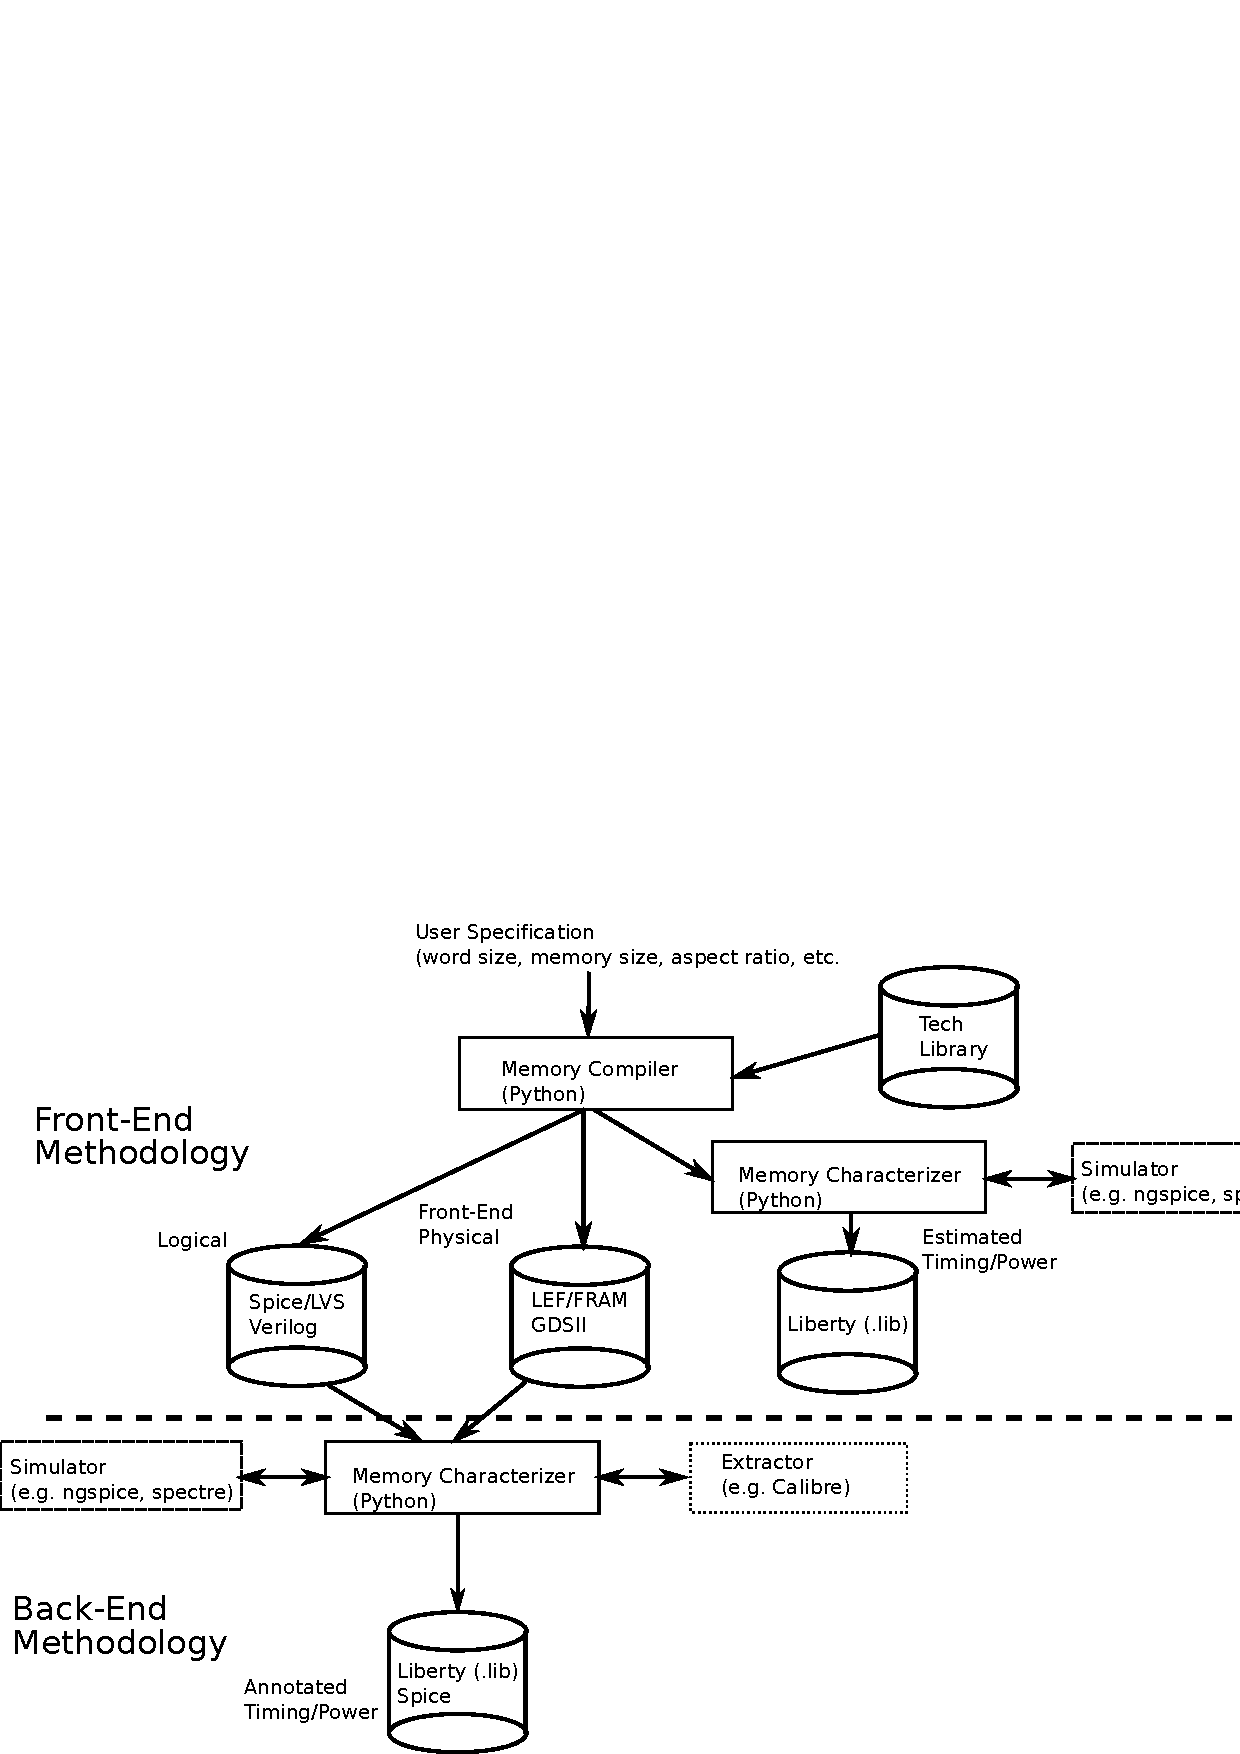
\includegraphics[width=14cm]{./figs/methodology.pdf}
\caption{Overall Compilation and Characterization Methodology
\label{fig:methodology}}
\end{figure}






